\documentclass{article}


\usepackage{arxiv}

\usepackage[utf8]{inputenc} % allow utf-8 input
\usepackage[T1]{fontenc}    % use 8-bit T1 fonts
\usepackage{hyperref}       % hyperlinks
\usepackage{url}            % simple URL typesetting
\usepackage{booktabs}       % professional-quality tables
\usepackage{amsfonts}       % blackboard math symbols
\usepackage{nicefrac}       % compact symbols for 1/2, etc.
\usepackage{microtype}      % microtypography
\usepackage{graphicx}
\usepackage{tikz}
\usepackage{circuitikz}
\usepackage{xurl}

\usetikzlibrary{positioning, shapes.geometric, arrows.meta}
\graphicspath{ {./images/} }


\title{\textsc{tabGPT}: Toward a Tabular Foundation Model}


\author{
 Felix Wick \\
  Panasonic R\&D Center Germany \\
  \texttt{felix.wick@eu.panasonic.com} \\
   \And
 Ulf Mertens \\
  Panasonic R\&D Center Germany \\
  \texttt{ulf.mertens@eu.panasonic.com} \\
   \And
 Naoki Setoguchi \\
  Panasonic Connect \\
  \texttt{setoguchi.naoki@jp.panasonic.com} \\
   \And
 Jun Matsuzaki \\
  Panasonic Connect \\
  \texttt{matsuzaki.jun001@jp.panasonic.com} \\
   \And
 Yoshito Tsuruda \\
  Panasonic Connect \\
  \texttt{tsuruda.yoshito@jp.panasonic.com} \\
   \And
 Ryuji Noda \\
  Panasonic Connect \\
  \texttt{noda.ryuji@jp.panasonic.com} \\
   \And
 Tawei Chang \\
  Panasonic Connect \\
  \texttt{chang.ta@jp.panasonic.com} \\
  %% \AND
  %% Coauthor \\
  %% Affiliation \\
  %% Address \\
  %% \texttt{email} \\
}

\begin{document}

\maketitle

\begin{abstract}
Transfer learning and foundation models have proven highly effective in domains involving homogeneous, unstructured data, such as computer vision and natural language processing. However, their application to structured or tabular data remains limited due to the inherent heterogeneity of such datasets. We propose a simple yet effective method for addressing the challenges associated with tabular data modeling by combining column embeddings generated with existing large language models and an encoder transformer architecture with a flexible prediction head. This approach integrates the vast knowledge of large language models with a robust numerical model backbone for pre-training across diverse datasets and tasks.
\end{abstract}


% keywords can be removed
%\keywords{First keyword \and Second keyword \and More}


\section{Introduction}
\label{sec:intro}

Transfer learning and foundation models based on deep learning methods are ubiquitous in the homogeneous, unstructured data regime, such as computer vision and natural language processing \cite{krizhevsky2012,dubey2024}. However, for structured or tabular data, its notorious heterogeneity hinders a widespread application \cite{grinsztajn2022}.

There are several compelling reasons why an effective tabular foundation model would be highly desirable:
\begin{itemize}
\item \textbf{Strong predictions with limited data}: By leveraging a pre-trained model, fine-tuning or even few-shot learning can yield accurate predictions, even with small training datasets.
\item \textbf{Leveraging LLM knowledge}: Such a model could benefit from the vast knowledge embedded in large language models (LLMs), enhancing its performance, especially in terms of data imputation.
\item \textbf{Feature learning}: It would also facilitate advanced feature learning, improving the model's ability to capture relevant patterns in the data.
\item \textbf{Data integration}: And arguably most importantly, it would solve the fundamental issue of data integration for tabular data sets, i.e., consolidating different data schemas and semantics, which requires quite some manual efforts in current models.
\end{itemize}

However, all current approaches struggle to fully address these requirements. In particular, the integration of extensive world knowledge from LLMs with a robust numerical model backbone for pre-training over various data sets and tasks remains a significant challenge.

\paragraph{Our Contributions}
We propose a simple approach, \textsc{tabGPT}\footnote{Code: \url{https://github.com/FelixWick/tabGPT}}, combining the following two ready-to-use components:
\begin{enumerate}
\item \textbf{Leveraging LLM for Column Embeddings}: We utilize an LLM to generate column embeddings, which facilitates consistent training across various datasets and tasks. This approach effectively addresses data integration challenges while incorporating the extensive knowledge and feature learning capabilities of LLMs.
\item \textbf{Transformer Backbone}: Our model employs a typical encoder-only transformer architecture with classification (or regression) head for making predictions. By omitting positional encoding, we preserve the permutation invariance of columns, enabling the model to directly input column embeddings into attention blocks. Additionally, we enhance our approach by incorporating a target/task description as an extra feature embedding, with positional encoding included for clear identification.
\end{enumerate}


\section{Related Work}
\label{sec:literature}

Current approaches may be classified into two broad categories, the ones utilizing pre-trained LLMs and tabular transformers \cite{schambach2024}. As we will describe in Section \ref{sec:method}, our proposed approach can be interpreted as combination of these two classes.

\subsection{Utilizing pre-trained LLMs}
Approaches utilizing pre-trained LLMs typically transform each row of a table into text, what is referred to as serialization. The produced text is then tokenized and fed into a pre-trained LLM. Thereby, each row is processed independently and in principle, this approach requires no dedicated training. But usually there is some fine-tuning of the used LLM on tabular tasks.

Architecture-wise, both encoder-only \cite{wang2024} and decoder-only \cite{hegselmann2023,wen2024,gardner2024} LLMs are possible, where at least the encoder-only LLMs require a head with a numeric loss, that needs to be fine-tuned. An advantage of the conditional generative nature of decoder models is the possibility of in-context learning, potentially interesting here in the form of few-shot prompting.

The serialization can also be done with an LLM, which can be another one than for the subsequent prediction step. There are different serialization formats and strategies, but generally, the column values are combined with the respective column name or an augmenting description.

While these methods solve the data integration issue of tabular data, LLMs pre-trained on text have inherent limitations in capturing complex numerical dependencies.

\subsection{Tabular Transformers}
In order to dedicatedly learn numerical correlations, one often adapts transformer-like architectures \cite{wang2022,zhu2023,hollmann2023} (or similarly graph attention networks \cite{kim2024}), because the permutation invariance of the self-attention mechanism reflects the arbitrary ordering of rows and columns in tabular data sets. It should be noted here that the causal masking used in transformer decoders partly destroy the permutation invariance of columns. So, encoder-only transformers without causal masking are preferable here.

The training across tables with different columns requires a mechanism to transform individual table rows into sequences of numerical representations. Usually, this is done with task-specific featurizers, which can be compared to embeddings in language models. A drawback of these approaches is that its featurizers need to be specified for each task, what makes it only partly practical as foundation model. Also, there is no mechanism to make use of the world knowledge of LLMs.

Another particular challenge of models for tabular data is how to treat numerical input values, especially continuous numbers, because its vector representations in a high-dimensional embedding space will hardly preserve the simple natural ordering. One possibility to overcome this issue is to use a single specific token for all numbers and multiply its learned embedding, i.e., vector representation, with the respective numerical value \cite{golkar2023}. Another, more flexible, possibility is to multiply the numerical values with the corresponding embedding of the column name or description \cite{kim2024}. However, this requires a tokenization that uses entire columns as individual tokens.


\section{Method}
\label{sec:method}

To overcome the limitations of the existing methods described in Section \ref{sec:literature}, we propose \textsc{tabGPT}, which consists of two steps: First, we generate numerical vector representations from the individual columns of the table for each row by means of an LLM, then we train an encoder-only transformer model with these column embeddings as inputs. An overview of \textsc{tabGPT} can be seen in Figure \ref{fig:tabGPT}.

\begin{figure}[ht]
    \centering
    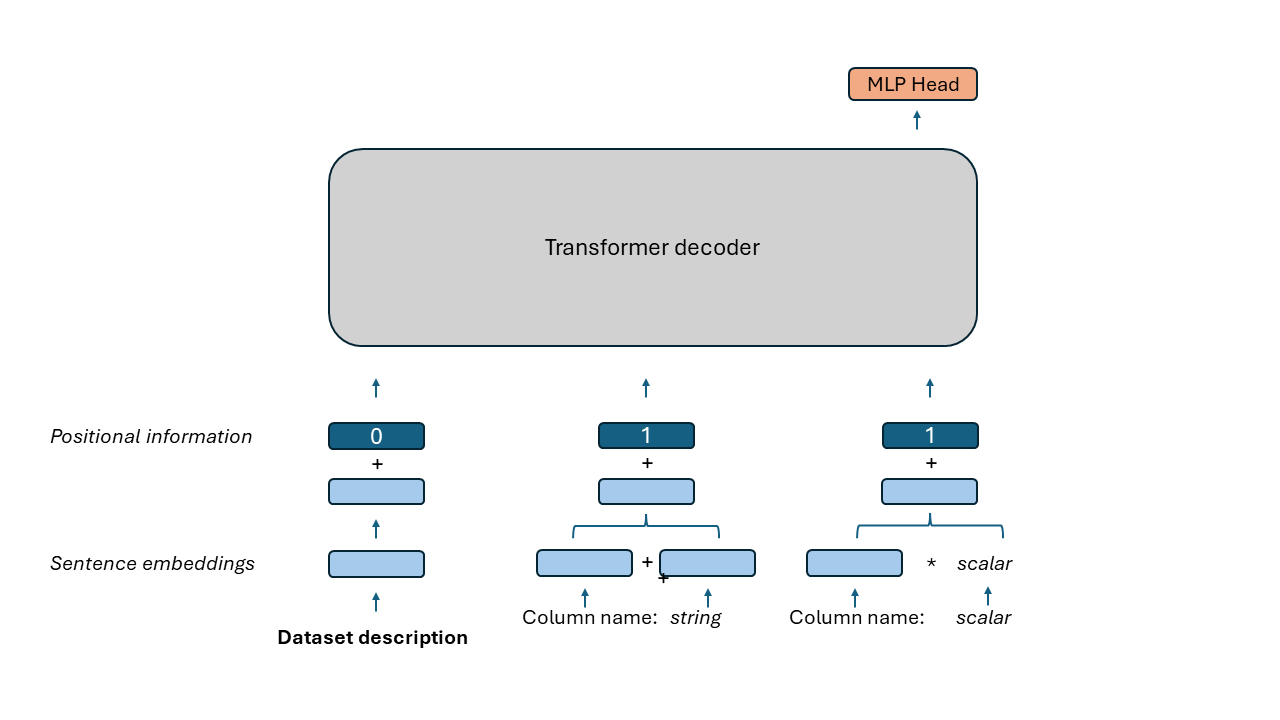
\includegraphics[width=0.95\linewidth]{tabgpt.png}
    \caption{Sketch of the \textsc{tabGPT} method. Externally generated sentence embeddings for dataset or target descriptions, column names or descriptions, and row values for categorical columns are used as inputs to an encoder-only transformer with a simple multi-layer perceptron (MLP) head for numerical predictions. Hereby, embeddings of categorical values are added element-wise and scalar numerical values are multiplied to the corresponding column embeddings for each row. Also, simple positional encodings are added only to distinguish the target embedding from the other inputs.}
    \label{fig:tabGPT}
\end{figure}

\subsection{Column Embeddings}
For each column in the dataset, we individually generate sentence embeddings. This process involves using the column name or, if available, an additional description as input to a forward pass through a \textsc{GPT-2} model (or any other text-generating LLM) pre-trained on language. We then extract the mean of the last hidden states for each token in the sequence, which forms the sentence embedding for that specific column.

For each row of the column at hand, we then combine the sentence embedding of the column name or description with the row value, where the exact combination depends on the nature of the values.

\subsubsection{Categorical Values}
\label{sec:categorical}
For categorical inputs, we perform the same embedding procedure as for the column names (or descriptions) for each unique category. Then we element-wise add the value embeddings for each row and the column name embeddings, where the latter are the same for each row.

\subsubsection{Numerical Values}
\label{sec:numerical}
For numerical inputs, we multiply each element of the column name embedding with the numerical value of the row at hand.

One difficulty lies in the treatment of zero values, because the multiplication with zero nullifies the column name embedding. A way to circumvent this is to use a dedicated category just for the zero value and follow the same procedure as for categorical values, i.e., embed the zero and add the resulting vector to the column embedding.

In order to generalize over different magnitudes of similar numerical columns in different data sets, it is beneficial to scale the numerical values to a given range. One possibility is to divide each value by the absolute value of the maximal positive or minimal negative value (whatever is larger) of the column.

\subsubsection{Target Encoding}
When training several data sets and tasks together, it is beneficial to include a target or task description in the model inputs to identify different target scales or model dynamics. For this, we perform the same embedding procedure as for the column names (or descriptions).

This can be interpreted as a way to kind of prompt the model at inference time to a specific task or target.

In order to distinguish the target embedding from the column embeddings, we add a simple positional encoding to the different vectors: 0 for the target and 1 for all the columns.

\subsection{Transformer Model}
The backbone for our proposed tabular foundation model is an encoder-only transformer, in our \textsc{tabGPT} implementation we use an architecture similar to \textsc{GPT-2}. But unlike typical language models, \textsc{tabGPT} operates without tokenization, embedding, and positional encoding. Instead it directly leverages the concatenation of the before created embeddings for each column along the sequence dimension.

To effectively generate predictions for classification or regression tasks, we replace the language model head with a classification or regression head and use a corresponding loss function (mean squared error for regression and cross-entropy for classification tasks). So far, we have trained different versions of \textsc{tabGPT} for regression and classification tasks, but in principle, one can use common model weights for all but the last layer.


\section{Experiments}
\label{sec:experiments}

As feasibility check for our proposed method, we conducted several experiments with our \textsc{tabGPT} implementation. In the following, we show its ability to generally predict tabular tasks, to work in a cross-training setup, and to create decent predictions with limited training data.

Some details about our implementation can be found in Appendix \ref{sec:minGPT}. All the models described in this section were trained from scratch, but it is possible to use language-pre-trained weights with our implementation.

\subsection{General-Purpose Usage}
\label{sec:single-task-exp}
Table \ref{tab:Kaggle_comp} shows the results of tabGPT for three different Kaggle competitions \cite{house-prices,store-sales,spaceship-titanic}. Details of the models and data sets can be found in Appendices \ref{sec:house-prices}, \ref{sec:store-sales}, and \ref{sec:titanic}. The comparisons with the respective Kaggle leaderboard results show that tabGPT can produce predictions with an accuracy similar to prevalent methods.

\begin{table}
 \caption{Results of our approach for three different Kaggle competitions, compared to the respective best leaderboard results, where we have dropped reported leaderboard results that seem unreasonable (probably due to target leakage in the test data sets). The evaluation metric for house prices \cite{house-prices} and store sales \cite{store-sales} is root mean squared logarithmic error (RMSLE), the one for spaceship Titanic \cite{spaceship-titanic} accuracy.}
  \centering
  \begin{tabular}{llll}
    \toprule
     & house prices & store sales & spaceship Titanic \\
    \midrule
    \textsc{tabGPT} & 0.138 & 0.450 & 79.9\% \\
    Kaggle leaderboard & 0.113 & 0.379 & 85.3\% \\
    \bottomrule
  \end{tabular}
  \label{tab:Kaggle_comp}
\end{table}

\subsection{Cross-Training}
\label{sec:cross-training}
The most important requirement for a tabular foundation model is that one can train across different data sets and tasks, i.e., tables with different columns and targets. To test this, we have performed a common training on four different regression tasks \cite{house-prices,store-sales,bicycles-count,demand-forecasting}. Details of the model and data sets can be found in Appendices \ref{sec:house-prices}, \ref{sec:store-sales}, \ref{sec:bicycles-count}, \ref{sec:demand-forecasting}, and \ref{sec:multi-task}.

The comparison of the results with the corresponding results of individual training, shown in Table \ref{tab:cross-training}, indicate that \textsc{tabGPT} can be trained across data sets and tasks without significantly loosing accuracy. It should be noted that there was no manual data integration needed to combine the different data sets in a common training.

\begin{table}
 \caption{Results of our approach for the test data sets of four different tasks \cite{house-prices,store-sales,bicycles-count,demand-forecasting}, once from a common cross-training, once from individual trainings on the corresponding training data sets only, and once from a fine-tuning on the respective training data set following a pre-training on the other three. Evaluation metric for all is RMSLE.}
  \centering
  \begin{tabular}{lllll}
    \toprule
     & house prices & store sales & bicycles count & demand forecasting \\
    \midrule
    cross-training & 0.19 & 0.23 & 0.34 & 0.62 \\
    individual training & 0.14 & 0.25 & 0.30 & 0.68 \\
    fine-tuning & ... & ... & ... & ... \\
    \bottomrule
  \end{tabular}
  \label{tab:cross-training}
\end{table}

\subsection{Fine-Tuning}
\label{sec:fine-tuning}
One of the key advantages of a tabular foundation model is the ability to produce good predictions with limited training data for a specific task, with the eventual goal of few-shot in-context learning, or even zero-shot learning. But this presumably requires lots of data sets and tasks with close similarities to be included in the training. On the other hand, a continuation of a training with a new data set or a split in a bigger pre-training on many tasks and data sets and a fine-tuning on a new and potentially small data set is feasible even with a small multi-task setup.

To show the effectiveness of the pre-train and fine-tune approach, we have repeated the cross-training experiment of Section \ref{sec:cross-training} four times, while always leaving one task out of the pre-training and fine-tune on it afterwards. The comparison of the results with the corresponding results of a pure pre-training are shown in Table \ref{tab:cross-training}.


\section{Conclusion and Outlook}
\label{sec:conclusion}

We propose \textsc{tabGPT}, a method to be used as backbone for a tabular foundation model. It consists of two parts, column embeddings generated from an LLM and an encoder-only transformer adapted for numerical predictions.

Please note that this is merely a proposal for the model architecture of a future foundation model, including some non-extensive feasibility studies. We neither state to have already built such a foundation model nor claim state-of-the-art performance. There is lots of work to be done toward a full tabular foundation model, especially in terms of data sets to be used for pre-training, but we hope this study will serve as an additional step in that direction.


\bibliographystyle{unsrt}  
%\bibliography{references}  %%% Remove comment to use the external .bib file (using bibtex).
%%% and comment out the ``thebibliography'' section.


%%% Comment out this section when you \bibliography{references} is enabled.
\begin{thebibliography}{1}

\bibitem{krizhevsky2012}
Alex Krizhevsky, Ilya Sutskever, and Geoffrey E. Hinton.
\newblock ImageNet classification with deep convolutional neural networks.
\newblock In {\em Proceedings of the 25th International Conference on Neural Information Processing Systems (NIPS)}, 2012, Volume 1, Pages 1097--1105.

\bibitem{dubey2024}
Abhimanyu Dubey et al.
\newblock The Llama 3 Herd of Models.
\newblock In {\em arXiv preprint}, 2024, arXiv:2407.21783 [cs.AI].

\bibitem{grinsztajn2022}
Léo Grinsztajn, Edouard Oyallon, and Gaël Varoquaux.
\newblock Why do tree-based models still outperform deep learning on tabular data?
\newblock In {\em Proceedings of the 36th International Conference on Neural Information Processing Systems (NIPS)}, 2022, Article No. 37, Pages 507--520.

\bibitem{schambach2024}
Maximilian Schambach.
\newblock Towards Tabular Foundation Models: Status quo, challenges, and opportunities.
\newblock In {\em HAL archive}, 2024, hal-04440710.

\bibitem{wang2024}
Zifeng Wang, Chufan Gao, Cao Xiao, and Jimeng Sun.
\newblock MediTab: Scaling Medical Tabular Data Predictors via Data Consolidation, Enrichment, and Refinement.
\newblock In {\em Proceedings of the 33rd International Joint Conference on Artificial Intelligence (IJCAI)}, 2024.

\bibitem{hegselmann2023}
Stefan Hegselmann, Alejandro Buendia, Hunter Lang, Monica Agrawal, Xiaoyi Jiang, and David Sontag.
\newblock TabLLM: Few-shot Classification of Tabular Data with Large Language Models.
\newblock In {\em Proceedings of The 26th International Conference on Artificial Intelligence and Statistics}, 2023, PMLR, Volume 206, Pages 5549--5581.

\bibitem{wen2024}
Xumeng Wen, Han Zhang, Shun Zheng, Wei Xu, and Jiang Bian.
\newblock From Supervised to Generative: A Novel Paradigm for Tabular Deep Learning with Large Language Models.
\newblock In {\em arXiv preprint}, 2024, arXiv:2310.07338 [cs.LG].

\bibitem{gardner2024}
Josh Gardner, Juan C. Perdomo, and Ludwig Schmidt.
\newblock Large Scale Transfer Learning for Tabular Data via Language Modeling.
\newblock In {\em arXiv preprint}, 2024, arXiv:2406.12031 [cs.LG].

\bibitem{wang2022}
Zifeng Wang and Jimeng Sun.
\newblock TransTab: Learning Transferable Tabular Transformers Across Tables.
\newblock In {\em Proceedings of the 36th International Conference on Neural Information Processing Systems (NIPS)}, 2022, Article No. 210, Pages 2902--2915.

\bibitem{zhu2023}
Bingzhao Zhu, Xingjian Shi, Nick Erickson, Mu Li, George Karypis, and Mahsa Shoaran.
\newblock XTab: Cross-table Pretraining for Tabular Transformers.
\newblock In {\em Proceedings of The 40th International Conference on Machine Learning}, 2023, PMLR, Volume 202, Pages 43181--43204.

\bibitem{hollmann2023}
Noah Hollmann, Samuel Müller, Katharina Eggensperger, and Frank Hutter.
\newblock TabPFN: A transformer that solves small tabular classification problems in a second.
\newblock In {\em The Eleventh International Conference on Learning Representations}, 2023.

\bibitem{kim2024}
Myung Jun Kim, Léo Grinsztajn, and Gaël Varoquaux.
\newblock CARTE: Pretraining and Transfer for Tabular Learning.
\newblock In {\em arXiv preprint}, 2024, arXiv:2402.16785 [cs.LG].

\bibitem{golkar2023}
Siavash Golkar, Mariel Pettee, Michael Eickenberg, Alberto Bietti, Miles Cranmer, Geraud Krawezik, Francois Lanusse, Michael McCabe, Ruben Ohana, Liam Parker, Bruno Régaldo-Saint Blancard, Tiberiu Tesileanu, Kyunghyun Cho, and Shirley Ho.
\newblock xVal: A Continuous Number Encoding for Large Language Models.
\newblock In {\em arXiv preprint}, 2023, arXiv:2310.02989 [stat.ML].

\bibitem{house-prices}
Anna Montoya, DataCanary.
\newblock House Prices - Advanced Regression Techniques.
\newblock Kaggle, 2016, \url{https://kaggle.com/competitions/house-prices-advanced-regression-techniques}

\bibitem{store-sales}
Alexis Cook, DanB, inversion, Ryan Holbrook.
\newblock Store Sales - Time Series Forecasting.
\newblock Kaggle, 2021, \url{https://kaggle.com/competitions/store-sales-time-series-forecasting}

\bibitem{spaceship-titanic}
Addison Howard, Ashley Chow, Ryan Holbrook.
\newblock Spaceship Titanic.
\newblock Kaggle, 2022, \url{https://kaggle.com/competitions/spaceship-titanic}

\bibitem{bicycles-count}
Department of Transportation (DOT).
\newblock Bicycle Counts for East River Bridges.
\newblock 2017, \url{https://data.cityofnewyork.us/Transportation/Bicycle-Counts-for-East-River-Bridges-Historical-/gua4-p9wg/about_data}

\bibitem{demand-forecasting}
Felix Wick.
\newblock 2023, \url{https://github.com/FelixWick/demand_forecasting_simulation}

\bibitem{minGPT}
Andrej Karpathy.
\newblock minGPT.
\newblock 2023, \url{https://github.com/karpathy/minGPT}

\end{thebibliography}


\newpage


\appendix

\section{\textsc{tabGPT} Implementation}
\label{sec:minGPT}

For ease of comprehension, we fork our \textsc{tabGPT} implementation from \textsc{minGPT} \cite{minGPT}, a popular, publicly available re-implementation of \textsc{GPT}.

As embedding or model dimension, we use \textsc{GPT-2} size of 768, reflecting our usage of \textsc{GPT-2} for column embeddings. The used number of layers and attention heads can differ for different models and are described below.

Compared to the original \textsc{minGPT} implementation, we made the following adaptions:
\begin{itemize}
\item no use of any tokenization, instead \textsc{GPT-2} call to generate sentence embeddings for column names or descriptions, categorical values, and target or task descriptions
\item dropped the causal masking in the self-attention mechanism to enable full permutation invariance of columns
\item dropped positional encodings, instead added simple positional encoding to distinguish column from target description embeddings
\item replaced language model head, loss function, and generation mechanism to reflect tabular prediction setup
\end{itemize}

In our implementation, there are different options for model configurations in terms of number of layers and number of self-attention heads. For all the experiments described here, we 4 layers and 4 self-attention heads. As embedding dimension, we use the one of \textsc{GPT-2}, which is 768.

\section{Data Set Details}

All data sets used for this work are openly available. We have put emphasis on regression tasks, both because there are underrepresented in former studies and are arguably more important for many real-world applications.

For the three Kaggle data sets, described below in \ref{sec:house-prices}, \ref{sec:store-sales}, and \ref{sec:titanic}, we use the train data sets for training and the test data sets for the predictions stated in the results, respectively.

As task or target descriptions, we simply use a short name for the described experiments: house prices, store sales, bicycles count, retail demand forecasting, spaceship titanic. In the multi-task mode described in Section \ref{sec:multi-task}, this helps to distinguish the different target scales and task dynamics. So, in a larger multi-task model, a more detailed description will be beneficial. In the single-task mode, it is completely irrelevant.

\subsection{House Prices}
\label{sec:house-prices}
As this is a regression task \cite{house-prices}, we use a typical MSE loss in the training. But we take the logarithm (to be exact, plus 1) of the target for the training, in order to optimize for the RMSLE metric used for the evaluation of the results.

We use all available 79 features for our model, without any feature engineering. We simply decide for each feature by its type whether it is used as categorical (see Section \ref{sec:categorical}) or numerical (see Section \ref{sec:numerical} one in our model. While the number of features is relatively large, the number of training samples is comparably low (1460 only), what makes it a challenging task.

Instead of the plain column names, we can alternatively use the column descriptions, as well as the descriptions of the different values for the categorical columns, which are provided on the web page, as input text for the column embeddings. While we anticipate this to be beneficial in a vast multi-task setup, it makes no significant difference in the single-task and small multi-task setup, especially when training from scratch without building on top of a language pre-training. So, we used the plain column and category names for our results here.

\subsection{Store Sales}
\label{sec:store-sales}
As this is a regression task \cite{store-sales}, we use a typical MSE loss in the training. But we take the logarithm (to be exact, plus 1) of the target for the training, in order to optimize for the RMSLE metric used for the evaluation of the results.

We perform some feature engineering to extract seasonality information from the date (namely the weekday, day in the month, and day in the year), compute the days before or after the most important holiday, and calculate an exponentially weighted moving average (EWMA) of the past sales for each store-family-weekday combination.

We use the following features as inputs for our model:
\begin{itemize}
\item categorical: \textsc{store}\textunderscore\textsc{nbr} (store), \textsc{family} (product group), weekday
\item numerical: \textsc{onpromotion} (items on promotion), \textsc{dcoilwtico} (oil price), day in month, day in year, days around Primer Grito de Independencia, EWMA of past sales
\end{itemize}

For the training, we only use data from May 2017 onward, because using earlier data did not improve the validation score.

\subsection{Spaceship Titanic}
\label{sec:titanic}
As this is a binary classification task \cite{spaceship-titanic}, we use a typical cross-entropy loss in the training.

We need to do some light feature engineering for this data set to extract the group information from the \textsc{PassengerID} column, which we use to build features reflecting the group size and number of individuals in the group. Similarly, we decompose the information in the \textsc{Cabin} column in cabin size and \textsc{deck}, \textsc{num}, \textsc{side}.

We use the following features as inputs for our model:
\begin{itemize}
\item categorical: single group or not, \textsc{deck}, \textsc{side}, single cabin or not, \textsc{HomePlanet}, \textsc{CryoSleep}, \textsc{Destination}, \textsc{VIP}
\item numerical: group size, number in group, cabin size, \textsc{num}, \textsc{Age}, \textsc{RoomService}, \textsc{FoodCourt}, \textsc{ShoppingMall}, \textsc{Spa}, \textsc{VRDeck}
\end{itemize}

\subsection{Bicycles Count}
\label{sec:bicycles-count}
As this is a regression task \cite{bicycles-count}, we use a typical MSE loss in the training. But we take the logarithm (to be exact, plus 1) of the target for the training, in order to optimize for the RMSLE metric used for the evaluation of the results.

We perform some light feature engineering to extract the weekday from the date and use the following features as inputs for our model:
\begin{itemize}
\item categorical: weekday, bridge
\item numerical: Precipitation, High Temp (F), Low Temp (F)
\end{itemize}

We use data from April 2017 until September 2017 for the training data set (732 rows), and from October 2017 for the test data set (124 rows).

\subsection{Demand Forecasting}
\label{sec:demand-forecasting}
We have simulated \cite{demand-forecasting} daily data points for 7 products and 3 stores from October 2021 until September 2022, where we use data until March 2022 for training (6374 rows) and data from April until September 2022 for testing (3302).

As this is a regression task, we use a typical MSE loss in the training. But we take the logarithm (to be exact, plus 1) of the target for the training, in order to optimize for the RMSLE metric used for the evaluation of the results.

We perform some light feature engineering to extract seasonality information from the date (namely the weekday, day in the month, and day in the year).

We use the following features as inputs for our model:
\begin{itemize}
\item categorical: product ID, product group ID, location ID, type of promotion, weekday
\item numerical: normal price, sales area, sales price, day in month, day in year
\end{itemize}

\subsection{Multi-Task Regression}
\label{sec:multi-task}
For our cross-training experiments, we combine the data sets described in Sections \ref{sec:house-prices}, \ref{sec:store-sales}, \ref{sec:bicycles-count}, and \ref{sec:demand-forecasting}, where we extend the data for \ref{sec:store-sales} to start from November 2016, but use only three stores (1, 2, and 3) and three product families (\textsc{LIQUOR,WINE,BEER}, \textsc{EGGS}, and \textsc{MEATS}), just to have a more balanced number of training samples for the different tasks. Also, in order to avoid lots of padding for the other data sets to get the same column dimension, we only use the 10 arguably most important features for \ref{sec:house-prices}, which does not change the quality of the model significantly.


\end{document}
